\section{Analysis}
\label{sec:Auswertung}

\subsection{Kontrast}
\label{sec:Kontrast}

In order to study the usage of interferrometrie to determine refraction indices, first of all the kontrast of the used Sagnac Interferometer was calculated.
The kontrast was calculated with equation \eqref{eq:K} and the values of table \ref{tab:Kontrast}.
Table \ref{tab:Kontrast} also contains the calculated kontrast values.
The maximum contrast K = 0.92 was measured at $\Phi = 130°$
Therefore the polarization filter was set to $\Phi = 130°$ for the following measurements.
In addition, a fit of the form 

\begin{equation}
  K = A \cdot |\text{cos}(\Phi) \text{sin}(\Phi)|
  \label{eq:fit}
\end{equation}
is performed with the mean values of the measured values.
This can be seen for the determined value of $A = 1.76 \pm 0.07$ in graph \ref{fig:Kontrast_Ausgleich}.

\begin{figure}[H]
  \centering
  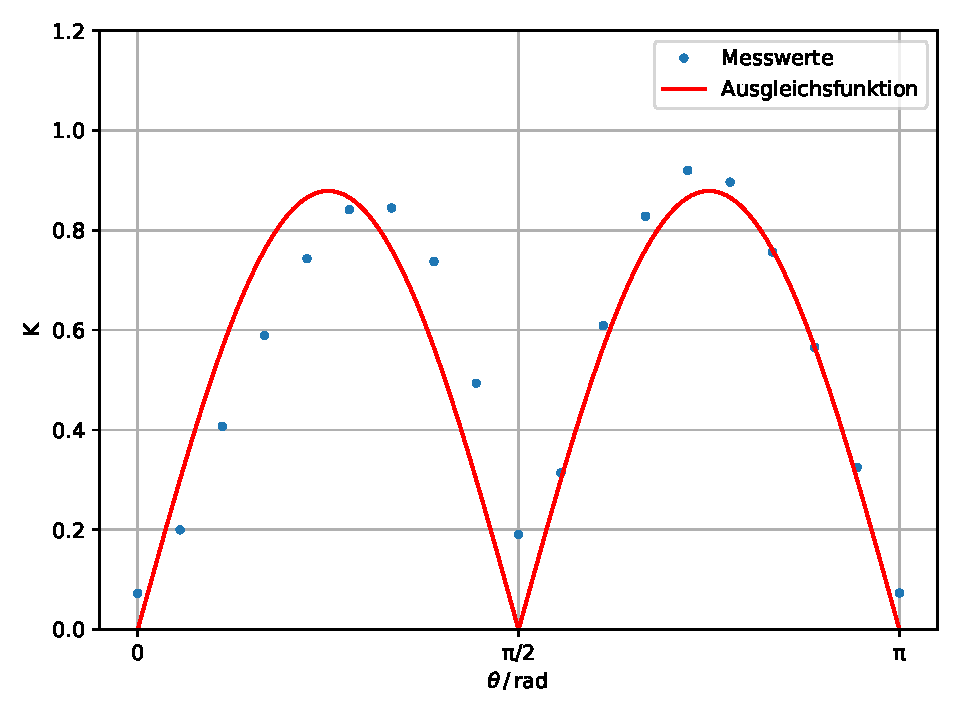
\includegraphics[width=\textwidth]{plots/kontrast_ausgleich.pdf}
  \caption{The measured values of the contrast according to equation \eqref{eq:K} and the fit calculation according to equation \eqref{eq:fit}.}
  \label{fig:Kontrast_Ausgleich}
\end{figure}

\begin{table}[H]
  \centering
  \caption{Recorded measured values for contrast measurement, as well as the respective contrast value.}
  \label{tab:Kontrast}
  \begin{tabular}{c c c c c c c c c c}
    \toprule
    $\Phi / \si{\degree} $ & $U_{\text{min,1}} / \si{\volt}$ & $U_{\text{max,1}} / \si{\volt}$ & $K_1$ & $U_{\text{min,2}} / \si{\volt}$ & $U_{\text{max,2}} / \si{\volt}$ & $K_2$ &  $U_{\text{min,3}} / \si{\volt}$ & $U_{\text{max,3}} / \si{\volt}$ & $K_3$ \\
    \midrule
    0  & 1.73 & 1.98 & 0.06 & 1.8  & 2.1  & 0.07 &  1.76 &  2.04 & 0.07 \\
    10 & 1.21 & 1.8  & 0.19 & 1.16 & 1.78 & 0.21 &  1.24 &  1.83 & 0.19 \\
    20 & 0.69 & 1.65 & 0.41 & 0.7  & 1.63 & 0.39 &  0.69 &  1.66 & 0.41 \\
    30 & 0.36 & 1.44 & 0.60 & 0.39 & 1.46 & 0.57 &  0.38 &  1.47 & 0.58 \\
    40 & 0.21 & 1.48 & 0.75 & 0.23 & 1.47 & 0.72 &  0.21 &  1.46 & 0.74 \\
    50 & 0.14 & 1.7  & 0.84 & 0.15 & 1.64 & 0.83 &  0.14 &  1.66 & 0.84 \\
    60 & 0.17 & 1.98 & 0.84 & 0.16 & 1.93 & 0.84 &  0.16 &  1.92 & 0.84 \\
    70 & 0.37 & 2.35 & 0.72 & 0.32 & 2.15 & 0.74 &  0.33 &  2.25 & 0.74 \\
    80 & 0.85 & 2.36 & 0.47 & 0.7  & 2.22 & 0.52 &  0.79 &  2.31 & 0.49 \\
    90 & 1.64 & 2.36 & 0.18 & 1.48 & 2.28 & 0.21 &  1.62 &  2.33 & 0.17 \\
    100& 1.43 & 2.93 & 0.34 & 1.46 & 2.68 & 0.29 &  1.49 &  2.79 & 0.30 \\
    110& 1.08 & 4.13 & 0.58 & 0.92 & 3.78 & 0.60 &  0.91 &  4.06 & 0.63 \\
    120& 0.52 & 5.06 & 0.81 & 0.49 & 5.06 & 0.82 &  0.44 &  5.36 & 0.84 \\
    130& 0.24 & 5.53 & 0.91 & 0.25 & 5.56 & 0.91 &  0.21 &  5.76 & 0.92 \\
    140& 0.34 & 5.92 & 0.89 & 0.33 & 5.91 & 0.89 &  0.3  &  5.99 & 0.90 \\
    150& 0.73 & 5.26 & 0.75 & 0.77 & 5.39 & 0.75 &  0.73 &  5.45 & 0.76 \\
    160& 1.16 & 4.13 & 0.56 & 1.22 & 4.25 & 0.55 &  1.16 &  4.38 & 0.58 \\
    170& 1.63 & 3.18 & 0.32 & 1.67 & 3.19 & 0.31 &  1.62 &  3.29 & 0.34 \\
    180& 1.86 & 2.08 & 0.05 & 1.85 & 2.18 & 0.08 &  1.79 &  2.11 & 0.08 \\
    \bottomrule
  \end{tabular}
\end{table}


\subsection{Refraction index of glas}
\label{sec:glas}

To determine the refractive index of glass, the number of intensity maxima M was recorded.
The refractive index was determined using the equation \eqref{eq:n}. 
The thickness of the plates is $D = 1$ mm, the wavelength of the laser  $\lambda_{\text{vac}} = 632.990$ nm. %and $\Omega_0 = 10°$ as the two plates are each $\Omega_0$ inclined.
The measured values, as well as the refractive index determined in each case, can be found in Table \ref{tab:Glas}.
On average, the refractive index determined for glass is
\begin{equation*}
  n_{\text{Glas}} = 1.64 \pm 0.13.
\end{equation*}

\begin{table}[H]
  \centering
  \caption{AMeasured values to determine the refractive index of glass and the determined refractive index.}
  \label{tab:Glas}
  \begin{tabular}{c c c}
    \toprule
    Durchgang & M & $n_\text{Glas}$ \\
    \midrule
    1    &  38  & 1.652 \\
    2    &  38  & 1.652 \\   
    3    &  38  & 1.652 \\   
    4    &  37  & 1.625 \\   
    5    &  38  & 1.652 \\   
    6    &  38  & 1.652 \\   
    7    &  37  & 1.625 \\   
    8    &  38  & 1.652 \\   
    9    &  38  & 1.652 \\   
    10   &  37  & 1.625 \\   
    \bottomrule
  \end{tabular}
\end{table}


\subsection{Refraction index of air}
\label{sec:air}

To determine the refractive index of air, the measured values were recorded as described in chapter \autoref{sec:Durchführung} and determined using equation \eqref{eq:n_air}.
The length of the gas chamber is L = (100.0 ± 0.1) mm and the temperature T = 20.6 °C .
The recorded values as well as the calculated reflection indices are shown in Table \ref{tab:Luft}.
%The average refractive index for each of the runs is listed in Table \ref{}.

%For the average refractive index, 
%\begin{equation}
%  n_{\text{Luft}} = 1.0002795 \pm 0.0000009,
%\end{equation}
%was determined.

\begin{table}[H]
  \centering
  \caption{Measured values recorded to determine the refractive index of air next to the refractive index calculated according to equation \eqref{eq:n_air}.
  Here, $M_i$ denotes the number of interference minima or maxima that have passed up to that point, where $i$ indicates the passage.}
  \label{tab:Luft}
  \begin{tabular}{c S[table-format=2.0] S[table-format=1.8] S[table-format=2.0] S[table-format=1.8] S[table-format=2.0] S[table-format=1.8] S[table-format=2.0] S[table-format=1.8]}
    \toprule
   {$p / \si{\milli\bar}$} & {$M_1$} & {$n_1$} & {$M_2$} & {$n_2$} & {$M_3$} & {$n_3$} & {$M_4$} & {$n_4$} \\
    \midrule
    50  & 2  & 1.00001266 & 2  & 1.00001266 &  2 & 1.00001266 & 3  & 1.00001899 \\
    100 & 4  & 1.00002532 & 4  & 1.00002532 &  4 & 1.00002532 & 5  & 1.00003165 \\
    150 & 7  & 1.00004431 & 6  & 1.00003798 &  6 & 1.00003798 & 7  & 1.00004431 \\
    200 & 9  & 1.00005697 & 8  & 1.00005064 &  8 & 1.00005064 & 9  & 1.00005697 \\
    250 & 11 & 1.00006963 & 10 & 1.00006330 & 10 & 1.00006330 & 11 & 1.00006963 \\
    300 & 13 & 1.00008229 & 12 & 1.00007596 & 12 & 1.00007596 & 13 & 1.00008229 \\
    350 & 15 & 1.00009495 & 15 & 1.00009495 & 15 & 1.00009495 & 15 & 1.00009495 \\
    400 & 17 & 1.00010761 & 17 & 1.00010761 & 17 & 1.00010761 & 18 & 1.00011394 \\
    450 & 20 & 1.00012660 & 19 & 1.00012027 & 19 & 1.00012027 & 20 & 1.00012660 \\
    500 & 22 & 1.00013926 & 21 & 1.00013293 & 21 & 1.00013293 & 22 & 1.00013926 \\
    550 & 24 & 1.00015192 & 23 & 1.00014559 & 23 & 1.00014559 & 24 & 1.00015192 \\
    600 & 26 & 1.00016458 & 25 & 1.00015825 & 25 & 1.00015825 & 26 & 1.00016458 \\
    650 & 28 & 1.00017724 & 27 & 1.00017091 & 27 & 1.00017091 & 28 & 1.00017724 \\
    700 & 30 & 1.00018990 & 30 & 1.00018990 & 29 & 1.00018357 & 30 & 1.00018990 \\
    750 & 32 & 1.00020256 & 31 & 1.00019623 & 32 & 1.00020256 & 33 & 1.00020889 \\
    800 & 35 & 1.00022155 & 34 & 1.00021522 & 34 & 1.00021522 & 35 & 1.00022155 \\
    850 & 37 & 1.00023421 & 36 & 1.00022788 & 36 & 1.00022788 & 37 & 1.00023421 \\
    900 & 39 & 1.00024687 & 38 & 1.00024054 & 38 & 1.00024054 & 39 & 1.00024687 \\
    950 & 41 & 1.00025953 & 40 & 1.00025320 & 40 & 1.00025320 & 41 & 1.00025953 \\
    \bottomrule
  \end{tabular}
\end{table}



\subsection{ Lorentz-Lorenz law}
\label{sec:Lorenz}

Since the refractive index also dependents on temperature and pressure according to the Lorentz-Lorenz law, an fit calculation is carried out according to equation \ref{eq:n_glas_taylor} .
The fit has the form 

\begin{equation}
  n = \frac{a}{TR} \cdot p + b
\end{equation}
The temperate is T = 20.6 °C and R describes the universal gas constant.
This results in the in table \ref{tab:ausgleich} shown values for a and b.

\begin{table}[H]
  \centering
  \caption{The results of the fit for the variables $a$ and $b$ for each run.}
  \label{tab:ausgleich} 
  \begin{tabular}{c c c}
    \toprule
    Messung & $a / \left(10^{-2} \si{\cubic\metre\per\mole} \right)$ & $b$ \\
    \midrule
    1    &  0.00066776 \pm 0.00000394 & 1.00000056 \pm 0.00000092 \\   
    2    &  0.00065800 \pm 0.00000397 & 0.99999789 \pm 0.00000093 \\   
    3    &  0.00065854 \pm 0.00000364 & 0.99999778 \pm 0.00000085 \\   
    4    &  0.00066017 \pm 0.00000370 & 1.00000344 \pm 0.00000086 \\
    \bottomrule
  \end{tabular}
\end{table}

The fits and thus the calculated refractive indices are shown in Figure \ref{fig:lorentz_lorenz} .
The average values for the variables are:

\begin{align*}
  a = 0.0006611 \pm 0.0000019 \frac{m^3}{\text{mol}}\\
  b = 0.9999999 \pm 0.0000004. \\
\end{align*}
According to the Loretz-Lorenz law, this results in the following refractive index in a normal atmosphere with T = 15 °C and p = 1013 hPa:
\begin{equation}
  n = 1.0002795 \pm 0.0000009
\end{equation}

\begin{figure}[H]
  \centering
  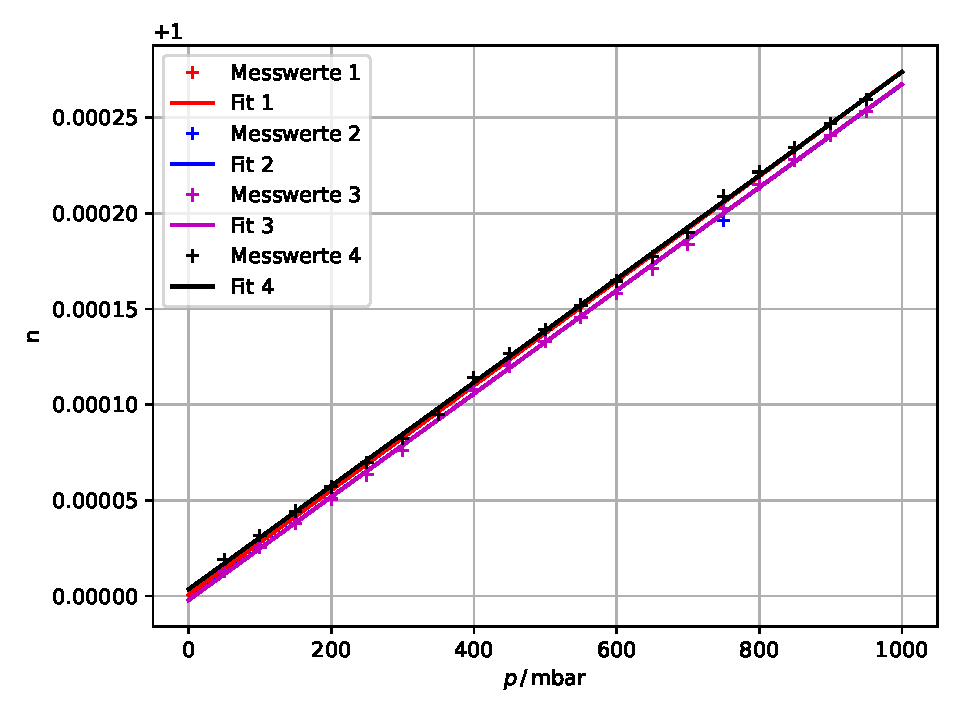
\includegraphics[width=\textwidth]{plots/lorentz_lorenz.pdf}
  \caption{The calculated refractive indices $n$ for air and the fit.}
  \label{fig:lorentz_lorenz}
\end{figure}


